\chapter{Figures} \label{app_2}

% 1. raw data EDA figures
\begin{figure}[]
	\begin{center}
		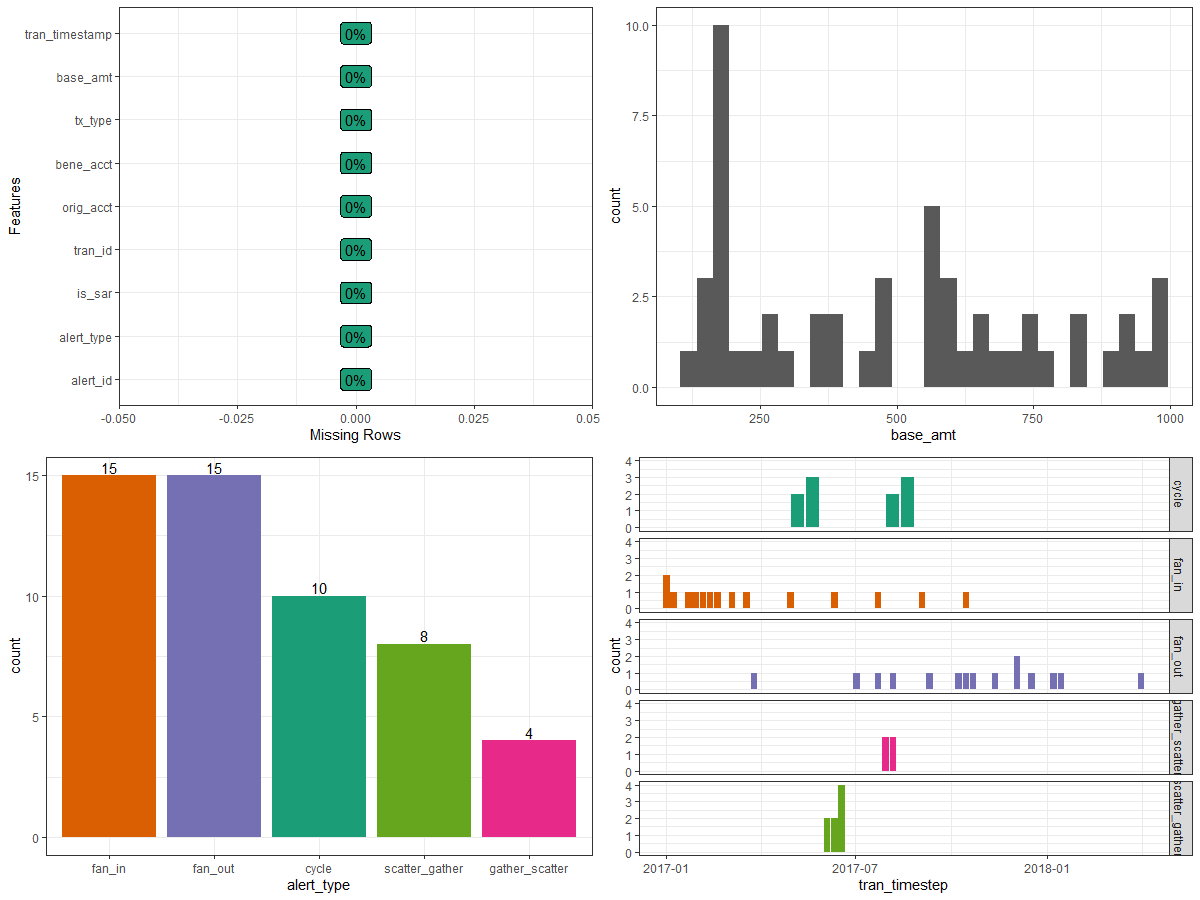
\includegraphics[scale=0.5]{fig/CH3/test_alrt_trans_summary.png}
		\caption{Example of the visualisations generated during the EDA of the test \texttt{alert\_transactions.csv} file. (top-left) The missing values profile. (top-right) Histogram of the transaction amount (\texttt{base\_amount}). (bottom-left) Frequency bar chart of the occurrences of different money laundering typologies (\texttt{alert\_type}) among the account transactions. (bottom-right) A timeline plot of when the different money laundering typologies occurred.}
		\label{fig:ch3_raw_eda_test_alrt_trans_sum}
	\end{center}	
\end{figure}

\begin{figure}[]
	\begin{center}
		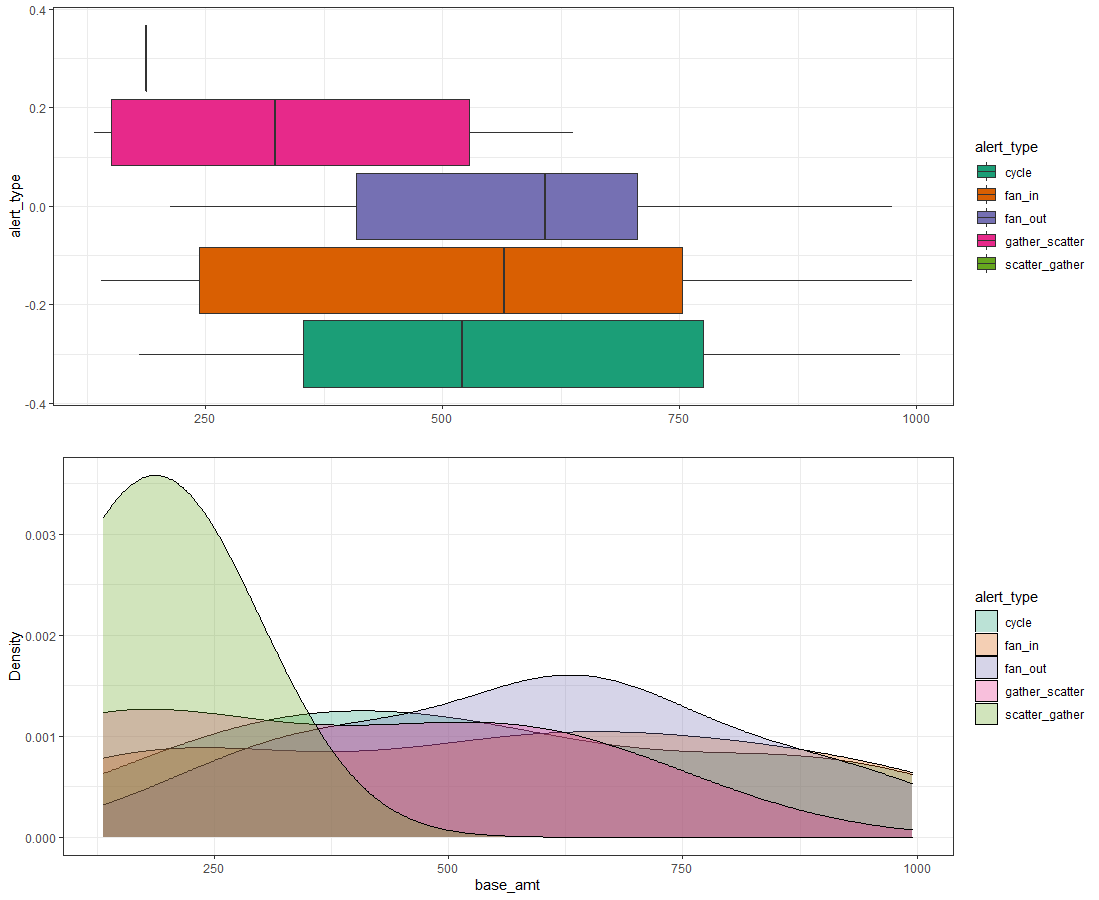
\includegraphics[scale=0.5]{fig/CH3/test_alrt_trans_tx_amount_alert_type_distribution.jpg}
		\caption{Both plots show the transaction amount distribution (top - box and whiskers and bottom - density plot) of transactions that were classified as being money laundering transactions for the test \texttt{alert\_transactions.csv} file.}
		\label{fig:ch3_raw_eda_test_alrt_trans_tx_distr}
	\end{center}	
\end{figure}

\begin{figure}[]
	\begin{center}
		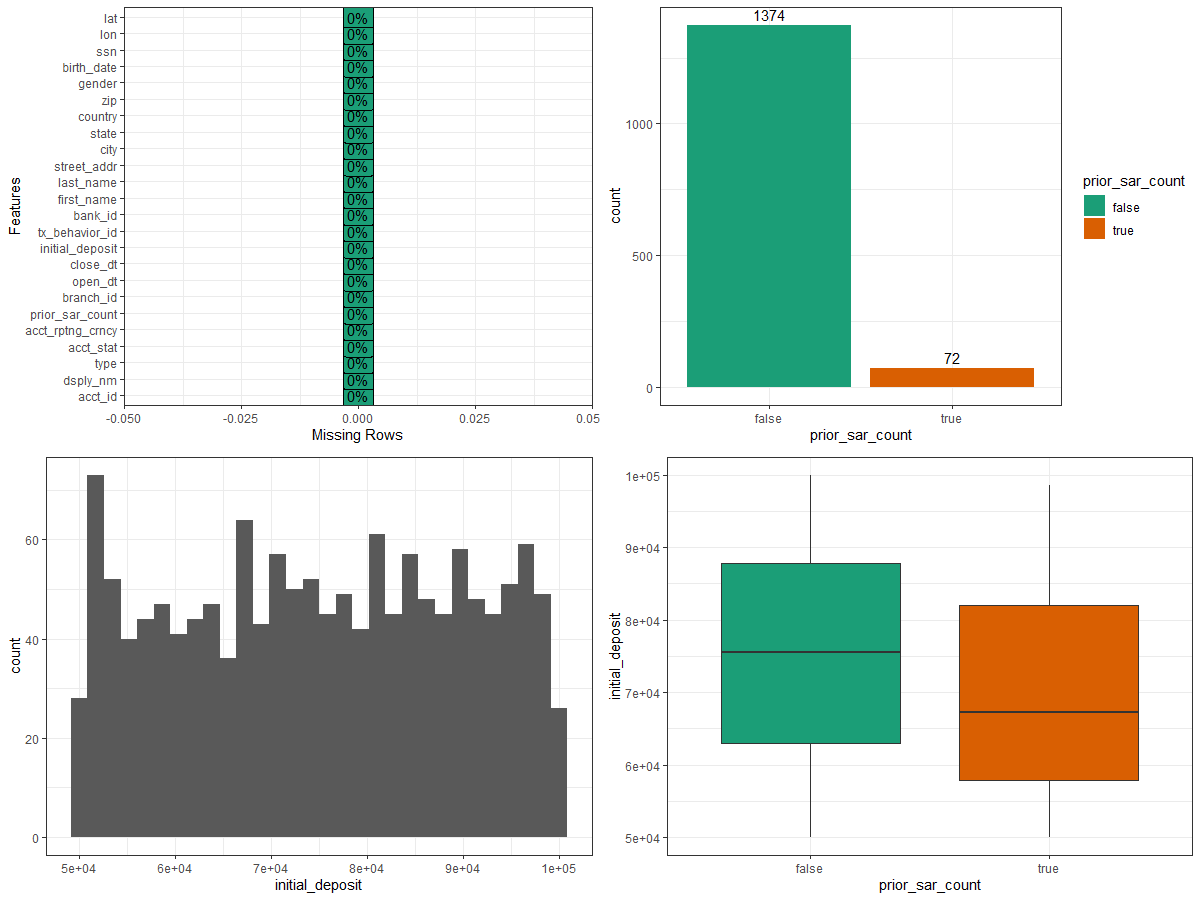
\includegraphics[scale=0.5]{fig/CH3/test_acc_summary.png}
		\caption{Example of the visualisations generated during the EDA of the test \texttt{accounts.csv} file. (top-left) The missing values profile. (top-right) Frequency bar chart of accounts that did and did not participate in money laundering activity. (bottom-left) Histogram of the accounts initial balances (\texttt{initial\_deposit}. (bottom-right) A box and whiskers plot showing money laundering and honest account's initial deposits.}
		\label{fig:ch3_raw_eda_test_acct_sum}
	\end{center}	
\end{figure}

% 2. 10-fold cross-validation lambda figures (transactional and combined)  
\begin{figure}[]
	\begin{center}
		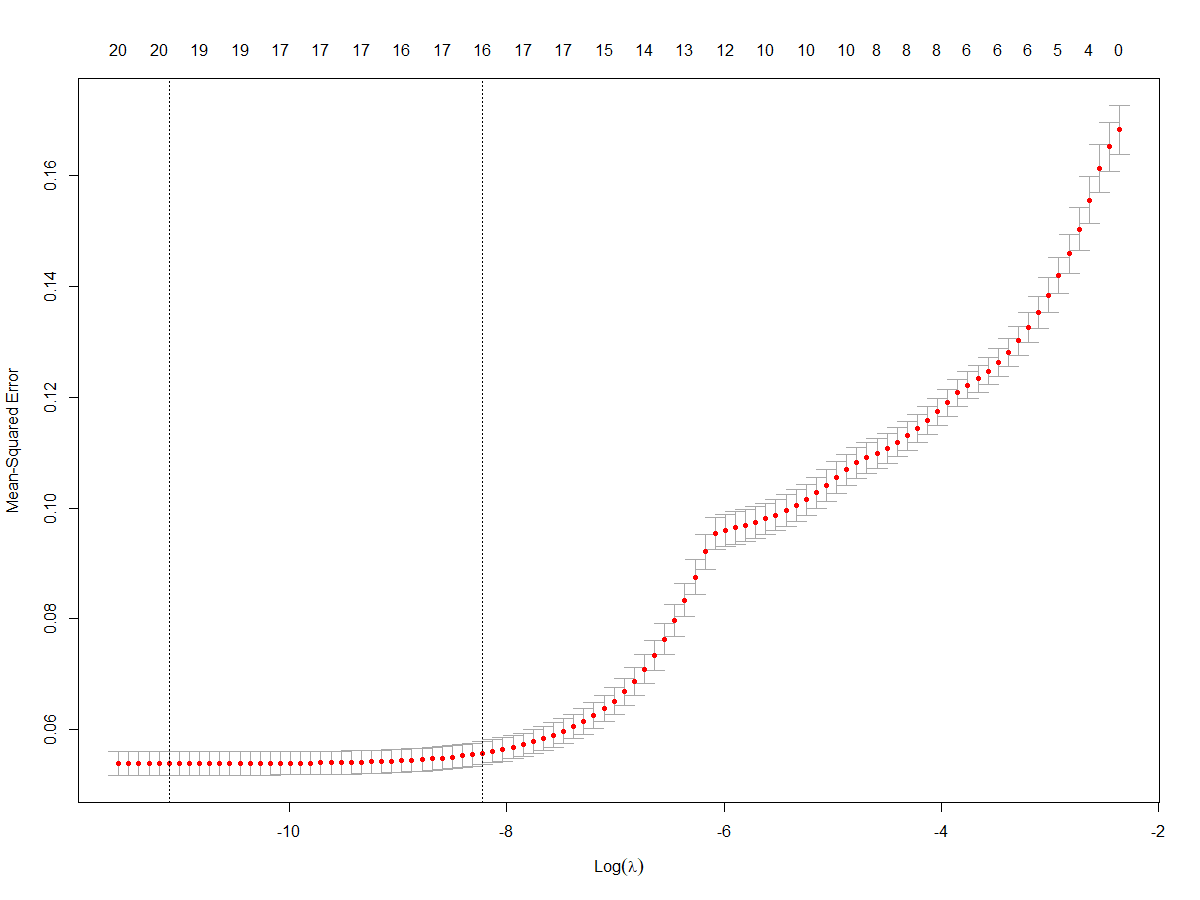
\includegraphics[scale=0.45]{fig/CH3/cv_lambda_trans.png}
		\caption{Ten-fold cross-validation mean square error (MSE) for the L1 regularised logistic regression model applied to the transactional feature data set. The vertical dashed line on the left is the $log(\lambda)$ value of where the MSE is at its minimum and the vertical on the right is the largest $log(\lambda)$ value such that the MSE is within one standard error of the minimum MSE. Also, the plot illustrates at the top, the number of positive weights $\boldsymbol{w} > 0$ at a specific $log(\lambda)$ value.}
		\label{fig:ch3_lr_lambda_cv_trans}
	\end{center}	
\end{figure}

\begin{figure}[]
	\begin{center}
		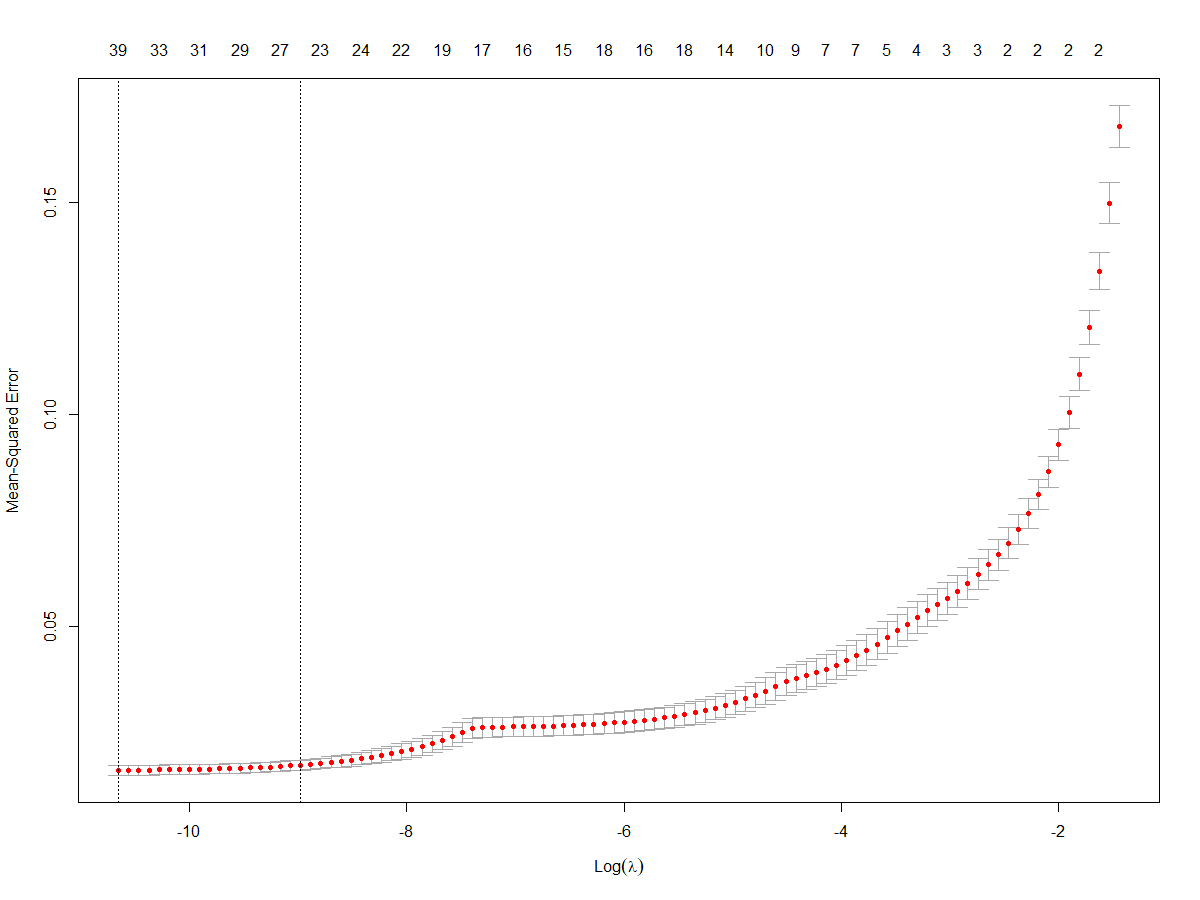
\includegraphics[scale=0.45]{fig/CH3/cv_lambda_all.png}
		\caption{Ten-fold cross-validation mean square error (MSE) for the L1 regularised logistic regression model applied to the combined feature data set. The vertical dashed line on the left is the $log(\lambda)$ value of where the MSE is at its minimum and the vertical on the right is the largest $log(\lambda)$ value such that the MSE is within one standard error of the minimum MSE. Also, the plot illustrates at the top, the number of positive weights $\boldsymbol{w} > 0$ at a specific $log(\lambda)$ value.}
		\label{fig:ch3_lr_lambda_cv_all}
	\end{center}	
\end{figure}

% validation curves NN -  (8)- transactional
\begin{figure}[]
	\begin{center}
		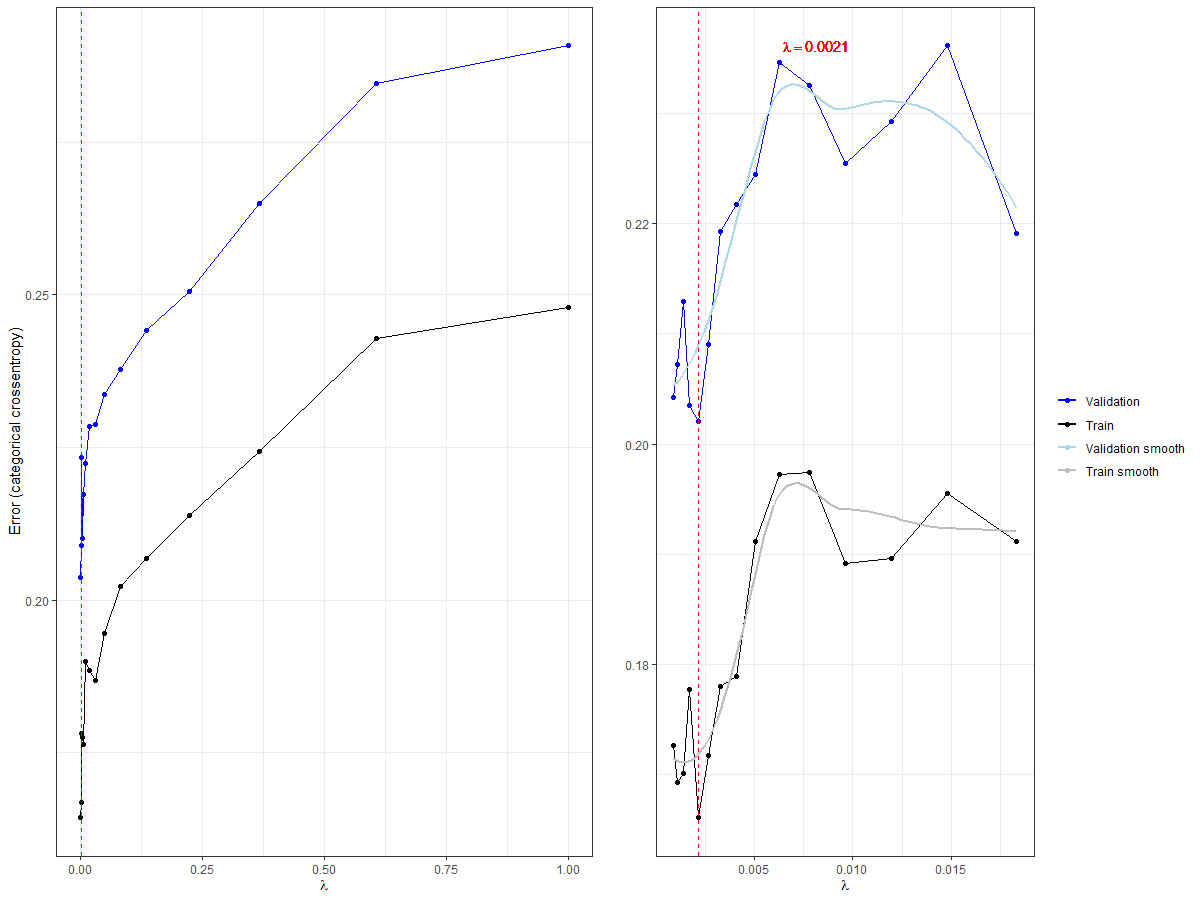
\includegraphics[scale = 0.5]{fig/CH3/trans_mod_1_lambda_plot.png}
		\caption{The plot illustrates the process of selecting the best approximate $\lambda$ value for the (8)-network model applied to the transactional feature data set. (left) The training and validation set errors for a range of $\lambda$ values. (right) The training and validation set errors for a more specific range of $\lambda$ values. The training and validation error smooth curves are additional curves to help view the curve patterns. Also, the $\lambda$ value that produced the minimum validation error is shown in both plots.}
		\label{fig:ch3_nn_validation_mod1_trans}
	\end{center}	
\end{figure}

% validation curves NN -  (64)- transactional
\begin{figure}[]
	\begin{center}
		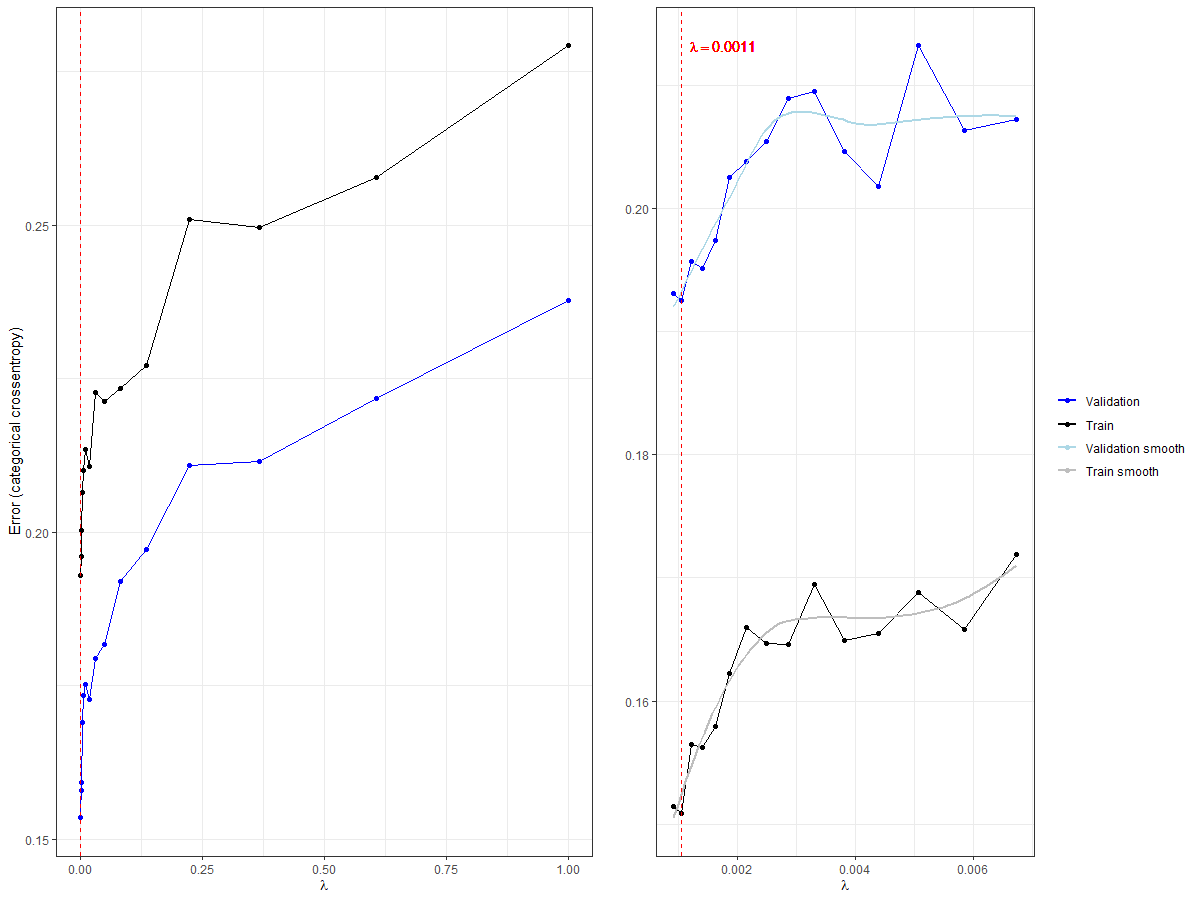
\includegraphics[scale = 0.5]{fig/CH3/trans_mod_2_lambda_plot.png}
		\caption{The plot illustrates the process of selecting the best approximate $\lambda$ value for the (64)-network model applied to the transactional feature data set. (left) The training and validation set errors for a range of $\lambda$ values. (right) The training and validation set errors for a more specific range of $\lambda$ values. The training and validation error smooth curves are additional curves to help view the curve patterns. Also, the $\lambda$ value that produced the minimum validation error is shown in both plots.}
		\label{fig:ch3_nn_validation_mod2_trans}
	\end{center}	
\end{figure}

% validation curves NN -  (8)- combines
\begin{figure}[]
	\begin{center}
		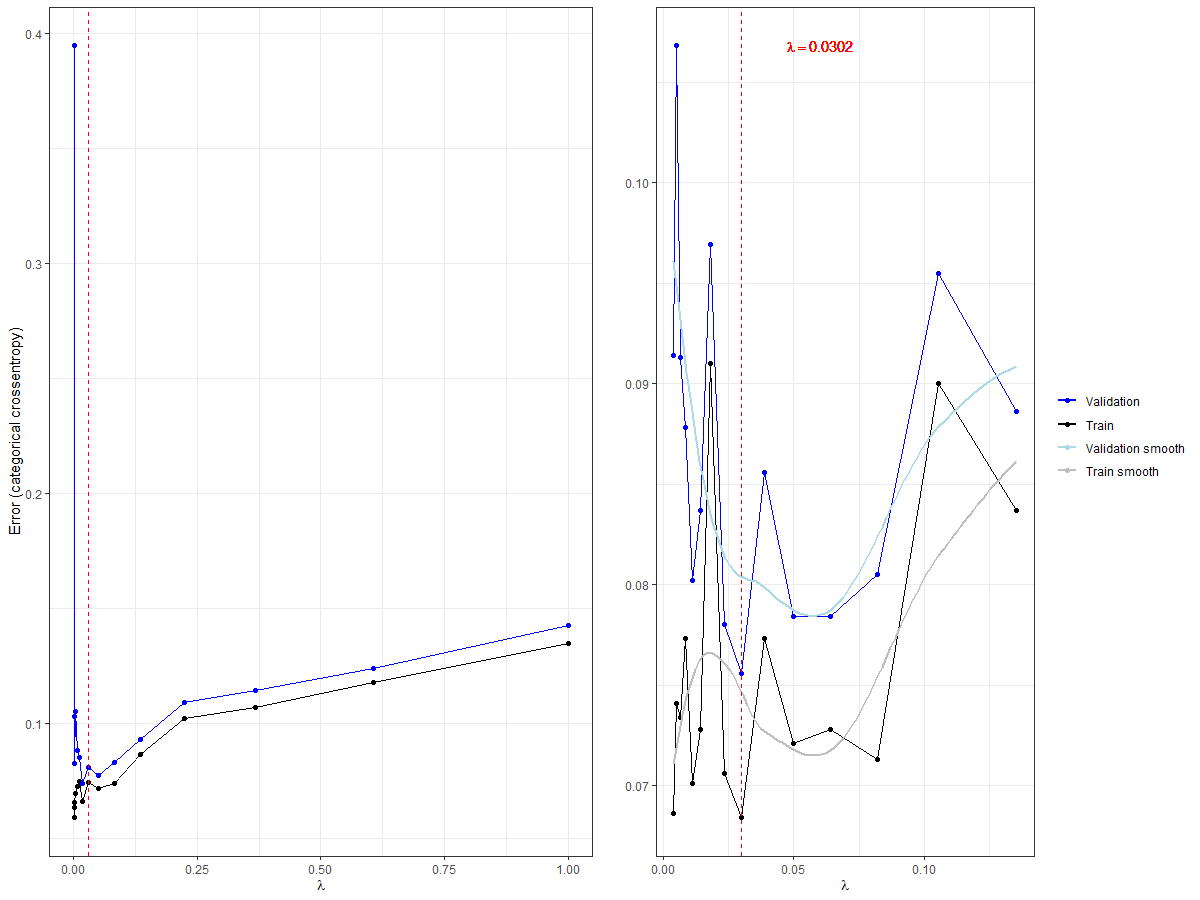
\includegraphics[scale = 0.5]{fig/CH3/all_mod_1_lambda_plot.png}
		\caption{The plot illustrates the process of selecting the best approximate $\lambda$ value for the (8)-network model applied to the combined feature data set. (left) The training and validation set errors for a range of $\lambda$ values. (right) The training and validation set errors for a more specific range of $\lambda$ values. The training and validation error smooth curves are additional curves to help view the curve patterns. Also, the $\lambda$ value that produced the minimum validation error is shown in both plots.}
		\label{fig:ch3_nn_validation_mod1_all}
	\end{center}	
\end{figure}

% validation curves NN -  (64)- all
\begin{figure}[]
	\begin{center}
		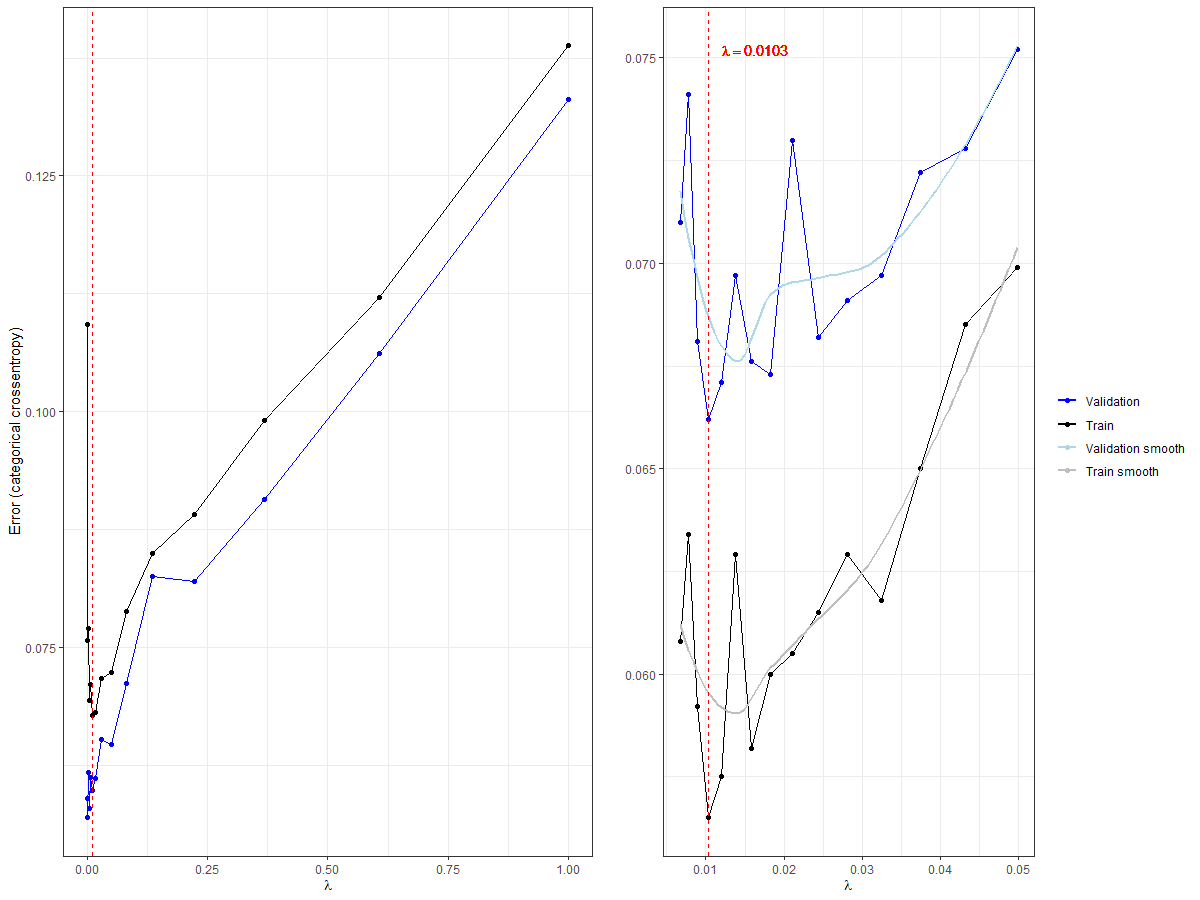
\includegraphics[scale = 0.5]{fig/CH3/all_mod_2_lambda_plot.png}
		\caption{The plot illustrates the process of selecting the best approximate $\lambda$ value for the (64)-network model applied to the combined feature data set. (left) The training and validation set errors for a range of $\lambda$ values. (right) The training and validation set errors for a more specific range of $\lambda$ values. The training and validation error smooth curves are additional curves to help view the curve patterns. Also, the $\lambda$ value that produced the minimum validation error is shown in both plots.}
		\label{fig:ch3_nn_validation_mod2_all}
	\end{center}	
\end{figure}

% validation curves comparison NN - transactional data
\begin{figure}[]
	\begin{center}
		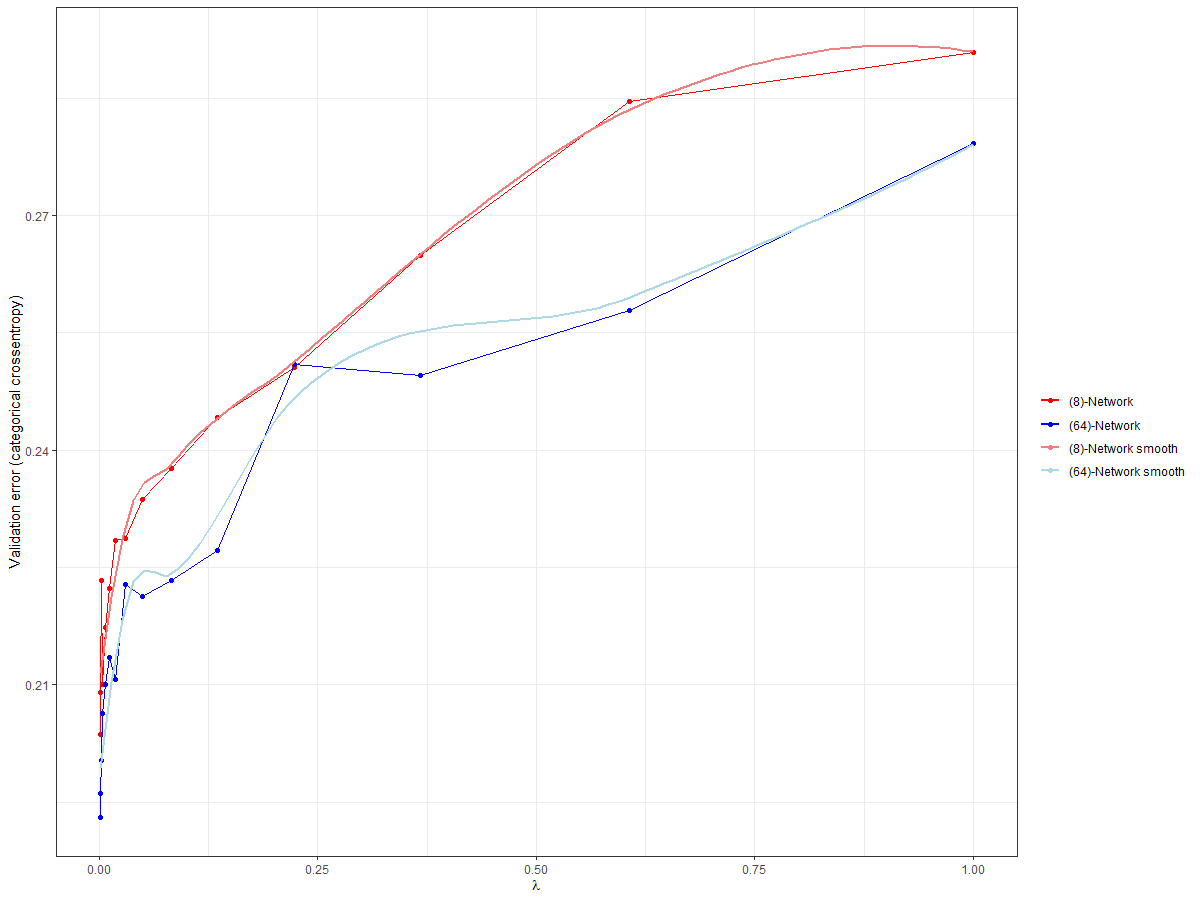
\includegraphics[scale = 0.5]{fig/CH3/model_comp_trans_HL_2.png}
		\caption{The superimposed validation error curves of the (8)-Network and (64)-Network models and their smoothing curves for $\lambda \in [0,1]$. Both models were applied to the transaction features data set.}
		\label{fig:ch3_nn_validation_compare_trans}
	\end{center}	
\end{figure}

% validation curves comparison NN - combined data
\begin{figure}[]
	\begin{center}
		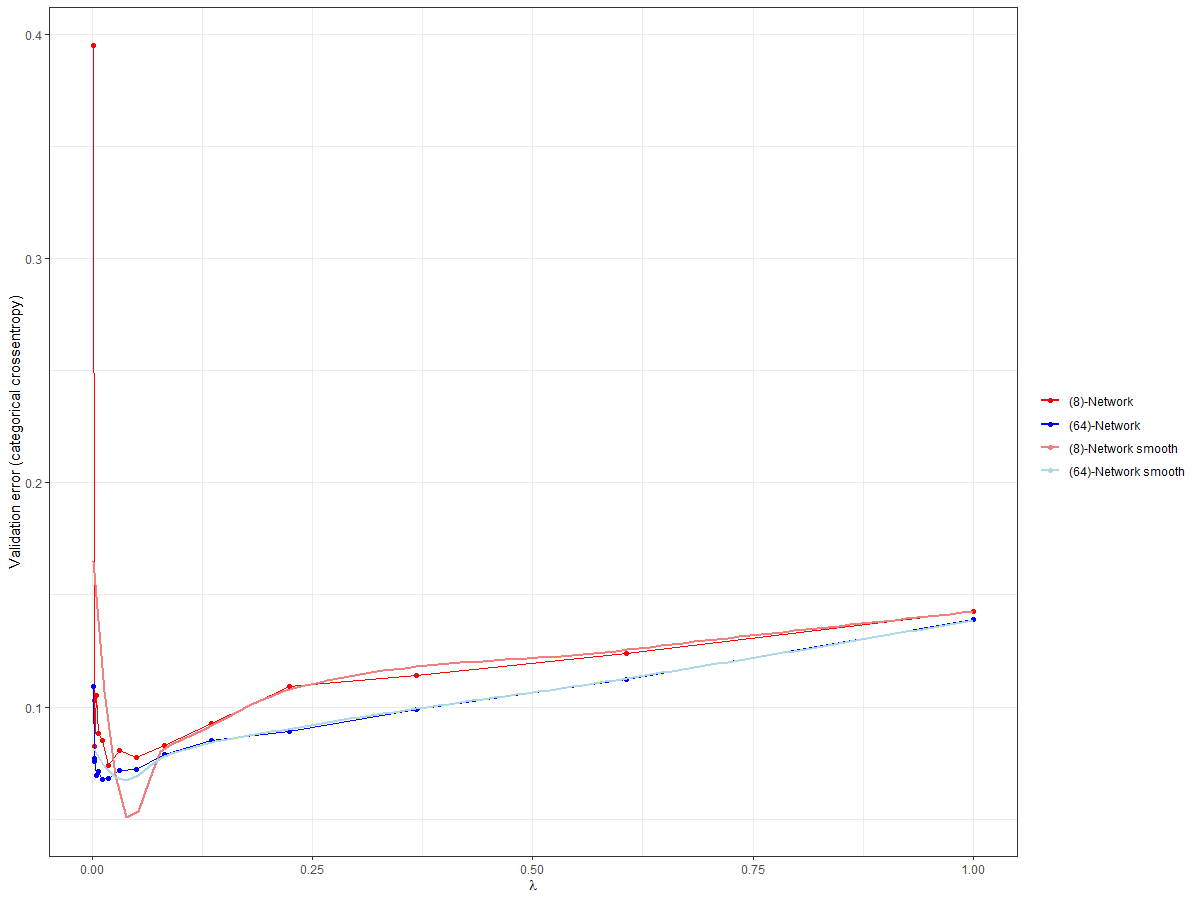
\includegraphics[scale = 0.5]{fig/CH3/model_comp_all_HL.png}
		\caption{The superimposed validation error curves of the (8)-Network and (64)-Network models and their smoothing curves for $\lambda \in [0,1]$. Both models were applied to the combined features data set.}
		\label{fig:ch3_nn_validation_compare_combined}
	\end{center}	
\end{figure}